\lhead{\textbf{Basic Algorithms, Fall 2024 \\ CSCI-UA.0310-001}}
\chead{\Large{\textbf{Homework 8}}}
\def\lc{\left\lceil}   
\def\rc{\right\rceil}
\rhead{\textbf{Instructor: Rotem Oshman \\Name: Ishan Pranav}}
\runningheadrule
\firstpageheadrule
\cfoot{}
\stepcounter{subsection}
\subsection*{References}
Peer-reviewed with Crystal Huang.

\subsection{Breadth-first search}
Recall the {\sc BFS} algorithm from the lecture that runs on graph $G$ starting from root node $s \in V$:
\begin{code}
    {\sc BFS}$(G,s)$\\
    1 \> $s.color = gray$, $s.dist = 0$. \\
    2 \> \For $u \in V \setminus \{s\}$ \\
    3 \> \> $u.color = white$, $u.dist = \infty$ \\
    4 \> $Q = \emptyset$ \\
    5 \> $Q.enqueue(s)$ \\
    6 \> \While $Q \neq \emptyset$ \\
    7 \> \> $u = Q.dequeue()$ \\
    8 \> \> \For $v \in Adj[u]$ \\
    9 \> \> \> \If $v.color = white$ \\
    10 \> \> \> \> $v.color = gray$ \\
    11 \> \> \> \> $v.dist = u.dist+1$ \\
    12 \> \> \> \> $Q.enqueue(v)$ \\
    13 \> \> $u.color = black$
\end{code}
\newpage
\begin{enumerate}
    \item Consider the undirected graph shown in Figure~\ref{fig:box}.
    If we begin a BFS traversal starting at node $A$, in what order are the nodes visited? Assume that the adjacency list is ordered alphabetically, i.e., we visit earlier letters alphabetically first, so from $A$ we will visit $B$ before $C$, and so on.
    
    \begin{figure}[h]
        \centering
        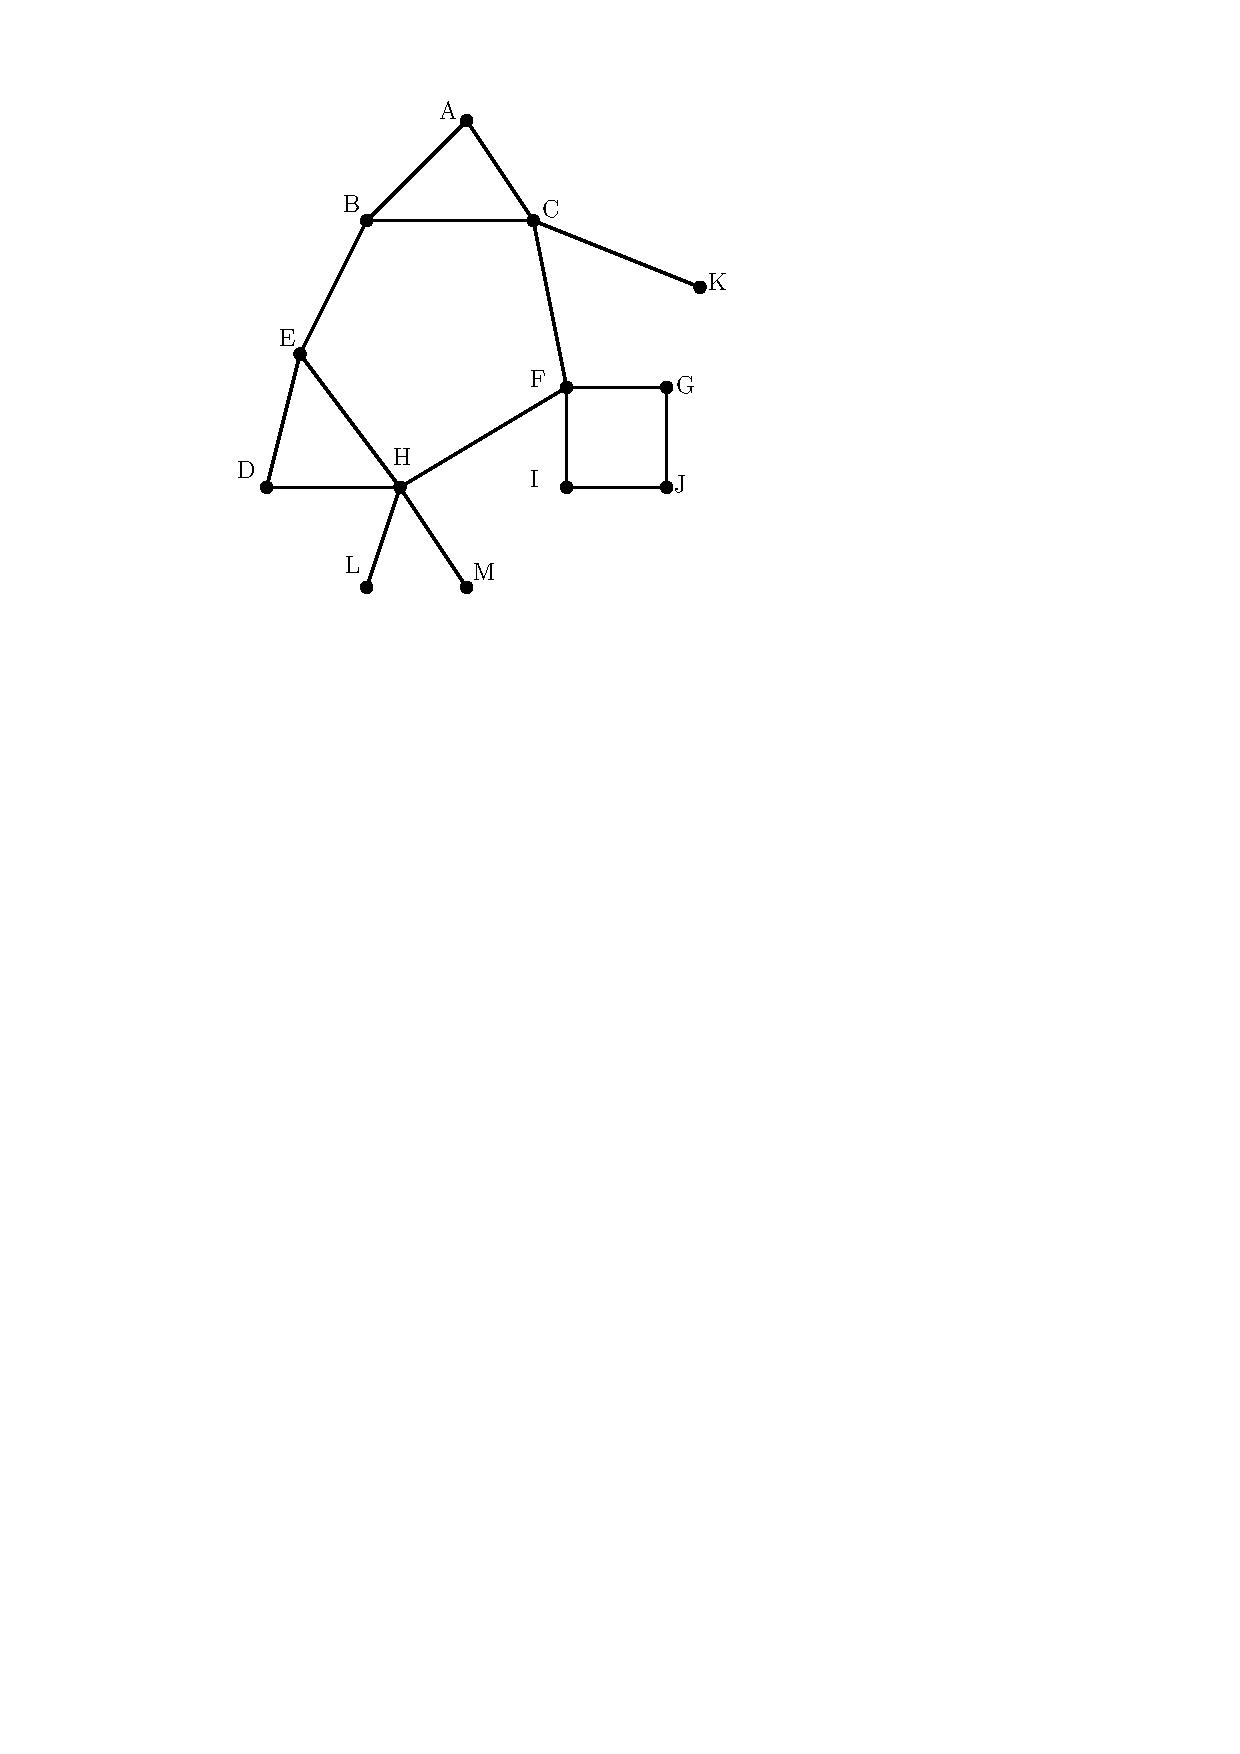
\includegraphics[width=0.4\textwidth]{images/BFS.pdf}
        \caption{Graph to traverse}
        \label{fig:box}
    \end{figure}
\begin{solution}
We can step through the breadth-first search algorithm to determine that the order of the vertices visited is A, B, C, E, F, K, D, H, G, I, L, M, and J.

\textit{First. }We enqueue A.

\textit{Second. }We dequeue A and enqueue B and C.

\textit{Third. }We dequeue B and enqueue E.

\textit{Fourth. }We dequeue C and enqueue F and K.

\textit{Fifth. }We dequeue E and enqueue D and H.

\textit{Sixth. }We dequeue F. We skip H. We enqueue G and I.

\textit{Seventh. }We dequeue K.

\textit{Eighth. }We dequeue H and enqueue L and M.

\textit{Ninth. }We dequeue G and enqueue J.

\textit{Tenth. }We dequeue I. We skip J.

\textit{Eleventh, twelfth, and thirteenth. }We dequeue L, M, and J.

The vertices are visited as enqueued: A, B, C, E, F, K, D, H, G, I, L, M, and J.
\end{solution}
\newpage
\item Explain what happens if we don't check whether a node is white before enqueuing it.
\begin{solution}
Suppose we did not check whether a node is white before enqueuing. Then the breadth-first search algorithm may not terminate.

For example, suppose we perform this variant of breadth-first search on graph $G=(V,E)$ with vertices $V=\{{\rm A},{\rm B},{\rm C}\}$ and edges $E=\{\{{\rm A},{\rm B}\}\}$. Assume, without loss of generality, that the initial vertex is A and that other vertices are visited in alphabetical order.

We can step through the algorithm to demonstrate the flaw.

\textit{First. }We enqueue A.

\textit{Second. }We dequeue A and enqueue B.

\textit{Third. }We dequeue B and enqueue A. Note that we enqueued A in this situation because we did not check its color and thus ignored the fact that it had been previously visited. 

This brings us back to the second step (dequeue A and enqueue B), meaning that the algorithm never terminates, even after all vertices have been visited.
\end{solution}
\newpage
\item Assume we replace the (FIFO) queue with a stack and therefore in line 7 obtain the node \emph{last} added. Does $v.dist$ still represent the shortest distance from $s$ to $v$?
\begin{solution}
No, using this implementation of breadth-first search, the distance assigned to a vertex $v$ may not represent the shortest distance from the starting vertex $s$ to $v$.

Consider the undirected graph $G=(V,E)$ with vertices $V=\{{\rm A},{\rm B},{\rm C},{\rm D},{\rm E}\}$ and edges $E=\{\{{\rm A},{\rm B}\},\{{\rm A},{\rm C}\},\{{\rm B},{\rm E}\},\{{\rm C},{\rm D}\},\{{\rm D},{\rm E}\}\}$. 

Assume, without los of generality, that the initial vertex is A and that other vertices are visited in alphabetical order.

We can see that the shortest path from A to E is $({\rm A},{\rm B},{\rm E})$, so the shortest distance from A to E is $2$.

However, if we step through the modified breadth-first search algorithm (a hybrid of breadth-first search and depth first search), we see that the algorithm handles the immediate children of the source node correctly, but mishandles its other descendent vertices.

\textit{First. }We push A with distance $0$.

\textit{Second. }We pop A, noting edges $\{{\rm A},{\rm B}\}$ and $\{{\rm A},{\rm C}\}$. We push B with distance $0+1=1$ and C with distance $0+1=1$.

\textit{Third. }We pop C, noting edge $\{{\rm C},{\rm D}\}$. We push D with distance $1+1=2$.

\textit{Fourth. }We pop D, noting edge $\{{\rm D},{\rm E}\}$. We push E with distance $2+1=3$. Already, this result is incorrect. We can continue stepping through the algorithm to show that it remains incorrect at termination.

\textit{Fifth. }We pop E.

\textit{Sixth. }We pop B, noting edge $\{{\rm B},{\rm E}\}$. We skip E.

The algorithm incorrectly assigns a distance of $3$ to E, although the shortest distance from A to E is $2$. We conclude that, in the modified algorithm, the distance assigned to $v$ is not necessarily the shortest distance from $s$ to $v$.
\end{solution}
\newpage
\item Consider graphs for which edges have assigned weights. Assume we modify line 11 of BFS to add the weight of the edge from $u$ to $v$ instead of adding $1$. Does the modified algorithm compute the shortest weighted distance correctly? If so, prove the correctness; otherwise, provide a counterexample for which the algorithm fails.
\begin{solution}
No, the modified algorithm is incorrect.

For example, suppose we perform this variant of the algorithm on graph $G=(V,E)$ with vertices $V=\{{\rm A},{\rm B},{\rm C},{\rm D}\}$ and edges $E$. For each edge $e\in E$, note $e=(u,v,w)$, where $u$ is the source vertex, $v$ is the target vertex, and $w$ is the weight of the edge. Suppose \[E=\{({\rm A},{\rm B},10),({\rm A},{\rm C},1),({\rm B},{\rm D},20),({\rm C},{\rm D},2)\}.\] Assume, without loss of generality, that $G$ is directed, that the initial vertex is A, and that other vertices are visited in alphabetical order.

We can step through the algorithm to demonstrate the flaw.

\textit{First. }We enqueue A with distance $0$.

\textit{Second. }We dequeue A, noting edges $({\rm A},{\rm B},10)$ and $({\rm A},{\rm C},20)$. We enqueue B with distance $0+10=10$ and C with distance $0+1=1$.

\textit{Third. }We dequeue B, noting edge $({\rm B},{\rm D},20)$. We enqueue D with distance $10+20=30$.

\textit{Fourth. }We dequeue C, noting edge $({\rm C},{\rm D},2)$. We skip D.

This gives $30$ for the distance from A to D by following path $({\rm A},{\rm B},{\rm D})$. However, there exists a path $({\rm A},{\rm C},{\rm D})$ whereby the distance from A to D is $3$. Of course, $3<30$. Thus, the modified algorithm fails.
\end{solution}
\end{enumerate}
\newpage
\subsection{Universal sink}
Recall that the \emph{adjacency matrix} representation of a \emph{directed} graph $G=(V,E)$ is the $|V| \times |V|$ matrix $M_G$ where $M_G[i][j]$ is $1$ if there is an edge from vertex $i$ to vertex $j$, and $0$ otherwise.
You may assume no vertex in the graph has an edge going into itself (i.e., no self-loops). We want to determine whether there is any vertex in $G$ that has edges coming to it from \emph{all other} vertices but no edges going out from it (this is known as a \textbf{universal sink}). 

\begin{enumerate}
\item Write an $O(|V|^2)$ algorithm that, given $M_G$, checks if there is a universal sink.
\begin{solution}

\textbf{Algorithm I. }{\sc IsSink}($M_G,v$) with a $|V|\times|V|$ adjacency matrix $M_G$ representing directed graph $G=(V,E)$ with no self-loops and a vertex $v\in V$; returns \verb|true| if $v$ is a universal sink; otherwise, \verb|false|:

For $u\in(V\setminus\{v\})$, if $M_G[v,u]=1$ or $M_G[u,v]=0$, then return \verb|false|.

Return \verb|true|.

\textbf{Algorithm II. }{\sc QuadraticSink}($M_G$) with a $|V|\times|V|$ adjacency matrix $M_G$ representing directed graph $G=(V,E)$ with no self-loops; returns \verb|true| if there is a universal sink in $G$; otherwise, \verb|false|:

For $v\in V$, if {\sc IsSink}($M_G,v$) is \verb|true|, then return \verb|true|.

Return \verb|false|.

\textbf{Proposition I. }\textit{Claim. }Algorithm I determines if $v$ is a universal sink in $G$ in running time $O(|V|)$.

\textit{Proof. }By definition, $v$ is a universal sink in $G=(V,E)$ if, for all $u\in V$ where $u\neq v$, we have $(u,v)\in E$ but $(v,u)\notin E$. The {\sc IsSink} algorithm compares $v$ to all other vertices $u$. It returns \verb|true| only if $v$ has edges coming to it from all other vertices $u$ and no edge going out from it to any vertex $u$. Otherwise, {\sc IsSink} returns \verb|false|. Thus, Algorithm I correctly determines if $v$ is a universal sink.

This implementation of Algorithm I visits every element in $V$ and performs constant-time operations within the loop body, so it has running time $O(|V|\times 1)=O(|V|).~\square$

\textbf{Proposition II. }\textit{Claim. }Algorithm II determines if there exists a universal sink in $G$ in running time $O(|V|^2)$.

\textit{Proof. }For $G=(V,E)$, The {\sc QuadraticSink} algorithm checks every vertex $v\in V$, using Algorithm I to determine if $v$ is a universal sink. From Proposition I, Algorithm I correctly determines if $v$ is a universal sink. Since Algorithm II returns \verb|true| if Algorithm I determines that any vertex is a universal sink (and \verb|false| if none satisfies this test), Algorithm II correctly determines if there exists a universal sink in $G$.

This implementation of Algorithm II visits every element in $V$ and performs {\sc IsSink} on each ($O(|V|)$ by Proposition I) within the loop body, so it has running time $O(|V|\times |V|)=O(|V|^2).~\square$
\end{solution}
\newpage
\item Write an $O(|V|)$ algorithm for the problem. Justify why it is correct, as well as why it satisfies this run-time bound.
\begin{solution}

\textbf{Algorithm III. }{\sc LinearSink}($M_G$) with a $|V|\times |V|$ adjacency matrix $M_G$ representing directed graph $G=(V,E)$ with no self-loops; returns \verb|true| if there is a universal sink in $G$; otherwise, \verb|false|:

If $V=\emptyset$, then return \verb|false|.

Let $v^*\leftarrow v\in V$, choosing $v$ arbitrarily.

Let $U\leftarrow V\setminus\{v^*\}$.

Let $W\leftarrow\emptyset$.

For $u\in U$:
\begin{itemize}
\item if $M_G[v^*][u]=1$ then:
\begin{itemize}
    \item assign $W\leftarrow W\cup\{v^*\}$;
    \item assign $v^*\leftarrow u$;
\end{itemize}
\item otherwise:
\begin{itemize}
    \item assign $W\leftarrow W\cup\{u\}$.
\end{itemize}
\end{itemize}

Return {\sc IsSink}($M_G,v^*$).

\textbf{Invariant I. }\textit{Claim. }For every step of the loop, no vertex $w\in W$ is a universal sink.

\textit{Proof. }We can prove this invariant by structural induction on $W$.

\textit{Basis. }Consider $W=\emptyset$. Then the invariant holds vacuously at initialization.

\textit{Hypothesis. }Consider $W=X$ where $X\neq\emptyset$. Assume there exists no universal sink $w\in W$.

\textit{Inductive step. }Consider $W=X\cup\{v\}$ for $v\in V$. From Algorithm III, there are two cases:
\begin{itemize}
\item Suppose $M_G[v^*][u]=1$. Then $v=v^*$ (before the reassignment of $v^*$). Thus $M_G[v][u]=1$, indicating that there is an outgoing edge from $v$, or $(v,u)\in E$. So $v$ is not a universal sink.
\item Suppose instead $M_G[v^*][u]=0$. Then $v=u$. Thus $M_G[v^*][v]=0$, indicating that there is no incoming edge to $v$, or $(v^*,v)\notin E$. So $v$ is not a universal sink.
\end{itemize}
In all cases, $v$ is not a universal sink.

For all $x\in X$, the invariant holds by the inductive hypothesis. Since the invariant holds for $v$, it must therefore hold for all vertices $w\in(X\cup\{v\})$.

Hence, by structural induction, there exists no universal sink $w\in W$. This invariant holds at initialization, maintenance, and termination.

\textbf{Proposition III. }\textit{Claim. }Algorithm III determines if there exists a universal sink in $G$ in running time $O(|V|)$.

\textit{Proof. }Suppose $V=\emptyset$. Then there is no universal sink in $G$, and Algorithm III returns \verb|false|, which is correct.

Suppose instead $V\neq\emptyset$. Then there exists an arbitrary $v^*\in V$. 

The loop executes for each of the $(|V|-1)$ elements in $U=V\setminus\{v^*\}$.

From Algorithm III, at initialization we have $|W|=0$. Also, for each iteration, exactly one element is inserted into $W$ in all cases. This implies that $|W|=(|V|-1)$ at termination. From Invariant I, at termination, we have for all $w\in W$ that $w$ is not a universal sink. Of course $v^*\notin W$, but $v^*\in V$. In fact, $v^*$ is the only vertex that has not been eliminated.

If $v^*$ is a universal sink, then there is a universal sink in $G$; otherwise, there is none.

Algorithm III returns $\textsc{IsSink}(M_G,v^*)$, which, by Proposition I, correctly determines if $v^*$ is a universal sink. Thus, Algorithm III correctly determines if there exists a universal sink in $G$.

The loop body performs constant-time operations in all cases, so the running time of the loop is $O((|V|-1)\times 1)=O(|V|-1)$. The running time of $\textsc{IsSink}(M_G,v^*)$ is $O(|V|)$ from Proposition I. Thus, the running time of \sc{LinearSink} is $O(|V|-1)+O(|V|)=O(|V|).~\square$
\end{solution}
\end{enumerate}
